\documentclass{article}
\usepackage{graphicx} % Required for inserting images
\usepackage{amsmath}
\usepackage{listings}
\usepackage{hyperref}
\usepackage{tikz}
\usepackage{pgfplots}

\title{Evidence 3 - Parallelizing a FFN-Layer}
\author{Moritz Trieu}
\date{May 2026}

\begin{document}

\maketitle

\section{Introduction}
The problem chosen was the calculation of a linear matrix combination $\mu(AX + b)$, where $A \in N \times M$,$x \in N \times M$ and $b \in N$. This computation is the basis of modern deep learning as it is the attribute computation in a feed-forwards layer as can be found in literature, for example in \cite{Goodfellow-et-al-2016}. In application $N$ and $M$ can be very large for example $N, M > 10,000$. In this case calculating the matrix product can be very demanding for a single core or thread. To speed up the process, the paradigm of parallelization was chosen. This splits up the operations onto different cores that can calculate different elements of the solution at the same time. In an optimal world this would reduce the computation time by the number of available cores $T_{\text{parallel}} = \frac{T_{\text{single}}}{N_{\text{cores}}}$. This is especially helpful if a large number of cores is available such as in GPUs.

\section{Model}
Splitting matrix addition into multiple parts is straight forward. Each thread can attach to one unique cell in the solution matrix, add the corresponding cells of the input matrices and write the solution into the corresponding matrix. Therefore, each cell can be extracted into an individual task. Thus the main challenge is the index linearization from the host matrix to the device  vector.

Matrix multiplication on the other hand becomes a bit more complicated. Calculating the $i_{th}$ component of the output vector is defined as $c_i = \sum_{j=0}^{M-1} a_{ij} \cdot x_{ji}$. Splitting up the task is for each matrix element of the output vector leaves each task with M operations. While easiest to implement it limits the distribution of work and each tasks workload scales with the size of the problem. 

\subsection{Linearization of Indices}
When copying matrices to the GPU memory, they get linearized row by row into an array as can be seen in Fig. \ref{fig:mat_lin}. The index mapping from matrix to vector can be calculated by $i_{vec} = i_{mat}\cdot N + j_{mat}$. From a visual standpoint this means a column index gets offset by the number of full rows prior. 

\begin{figure}
    \centering
    \begin{equation*}
        \begin{bmatrix}
            a_{11} & \dots & a_{1N} \\
            a_{21} & \dots & a_{2N} \\
            \vdots & \ddots & \vdots \\
            a_{N1} & \dots & a_{NN}
        \end{bmatrix} \xrightarrow{} 
        \begin{bmatrix}
            a_{11} & \dots & a_{1N} &
            a_{21} & \dots & a_{2N} &
            \dots &
            a_{N1} & \dots & a_{NN}
        \end{bmatrix}
    \end{equation*}
    \caption{Linearizing a matrix by appending each row onto the previous.}
    \label{fig:mat_lin}
\end{figure}

In the case of CUDA, each core also uses threads. Still, it might hold true, that the problem size bigger than the number of available threads. In this case we need a way to assign tasks without the possibility of threads overlapping tasks. To this end, we first need the global thread ID which can be calculated using $i_{\text{global}} = i_{\text{thread}} + i_{\text{block}} \cdot d_{\text{block}}$. The dimension of a block is the number of threads per block. So the local ID is comprised of the global amount of threads per core before with the local thread ID. To assign to this thread a new task, we can add the number of globally available threads, so we shift the global position by the entire size of the thread pool. This can be done until the size of the problem is reached as is visible in Lst. \ref{lst:pool}.

\begin{lstlisting}[mathescape=true, language=C++, caption=Assignment of threads when the problem size is bigger than the available pool. $\label{lst:pool}$]
int idx = threadIdx.x + blockIdx.x * blockDim.x;

int i = idx;
while (i < vec_size) {
    ...;
    i += blockDim.x * gridDim.x;
}
\end{lstlisting}

Each block is limited to a number of threads as specified in \cite{cuda2026}. This means one has to increase the number of blocks. Since each block has an integer ID, the number of IDs are limited. In big problems with a large amount of cores, where these IDs are not sufficient, one can make the threads 2 dimensional, squaring the number of available IDs. In this case, the global thread ID can be calculated by first calculating the global row and column index from the thread and block IDs which then in turn can be used to calculate the global thread ID as can be seen in in Lst. \ref{lst:2dblock}

\begin{lstlisting}[mathescape=true, language=C++, caption=Computing the global thread ID in the case of 2D blocks. $\label{lst:2dblock}$]
int row = threadIdx.x + blockIdx.x * blockDim.x;
int column = threadIdx.y + blockIdx.y * blockDim.y;

int thread_id = row * M + column;
while (thread_id < N*N) {
    ...;
    thread_id += blockDim.x * gridDim.x;
}

\end{lstlisting}

\section{Implementation}
The C++ implementation can be found in the file Evidence\_3\_Matmul\_parallel.ipynb 
(\url{TC2037-Evidence-3/blob/main/Evidence\_3\_Matmul\_parallel.ipynb}).

The element-wise matrix multiplication implementation can be found in Lst. \ref{lst:matmul}. An important observation is the linearization of indices to account for the different directions of index movement.

\begin{lstlisting}[mathescape=true, language=C++, caption=Element-wise matrix multiplication. $\label{lst:matmul}$]
float sum = 0;
for (int j= 0; j<M; j++) {
  sum += a[i * M + j] * x[i + j * N];
}
\end{lstlisting}

Another important aspect is variable definition and memory allocation on both device and host, as well as the setup of 2 dimensional blocks which can be seen in Lst. \ref{lst:dim3}.

\begin{lstlisting}[mathescape=true, language=C++, caption=Setup of 2D blocks using dim3. $\label{lst:dim3}$]
dim3 blocks_multi((N / THREADS) / 2, (N / THREADS) / 2);
dim3 threads_multi(THREADS, THREADS);
matmult << <blocks_multi, threads_multi >> >(d_a, d_b, d_x, d_c, N, M);
\end{lstlisting}


\section{Test}
To test the algorithm three different tests are run. 

The first test uses a small example of $N=4$, $M=2$ with an anisotropic number of blocks and smaller number of threads than tasks. This small example serves the purpose of testing (visually) if the result is correct and is testing the equation
\begin{equation}
    \begin{bmatrix}
        1&1\\
        1&1\\
        0&0\\
        0&0\\
    \end{bmatrix}
    \begin{bmatrix}
        1&1&1&1\\
        0&0&0&0
    \end{bmatrix}
    = \begin{bmatrix}
        1&1&1&1\\
        1&1&1&1\\
        0&0&0&0\\
        0&0&0&0
    \end{bmatrix}
\end{equation}

The second test measures the speed difference between single-core and multi-core for different problem sizes. The problem base size is $N = 4096$ and $M = 1024$ and is reduced by powers of 2. The number of threads for the multi-core case is kept constant at 256 with the number of blocks adapting to the problem of the size. The results can be seen in Fig. \ref{fig:singlevmulti}. It can be seen that with increasing problem size the time saving approaches roughly the number of threads. This is the expected behavior. In the implementation notebook, the startup time is also measured, which includes memory allocation, initialization and copying. It can be observed that the start-up time makes up the largest amount of time with increasing problem size and therefore places a limiting factor. 

The third test compares the runtime of using an increasing amount of threads with a constant problem size of $N = 4096$ and $M = 1024$. The resulting data can be seen in Fig. \ref{fig:threads} and shows a decrease in runtime with increasing threads as expected.

\begin{figure}
    \centering
    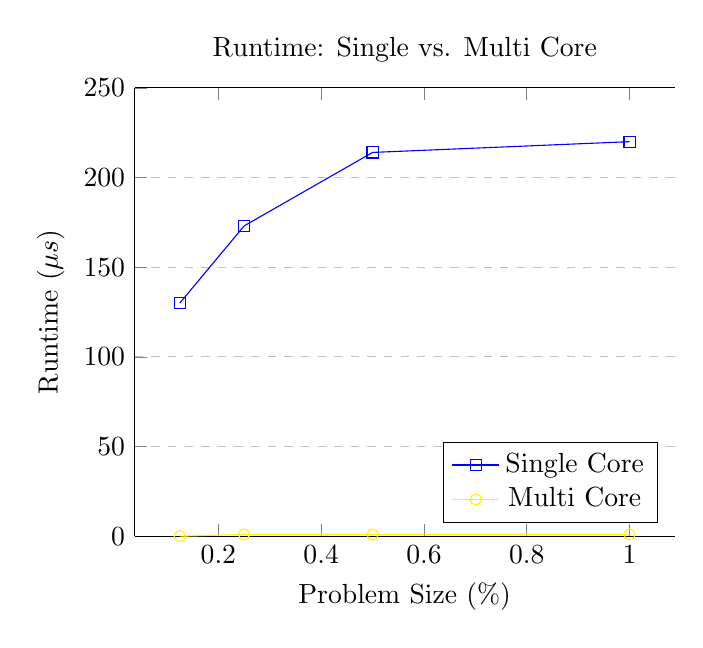
\begin{tikzpicture}
    \begin{axis}[
        title={Runtime: Single vs. Multi Core},
        xlabel={Problem Size (\%)},
        ylabel={Runtime ($\mu s$)},
        %xmin=0, xmax=100,
        axis y line*=left,
        ymin=0, ymax=250,
        %xtick={0,20,40,60,80,100},
        %ytick={0,20,40,60,80,100,120},
        legend pos=south east,
        ymajorgrids=true,
        grid style=dashed,
    ]
    
    \addplot[
        color=blue,
        mark=square,
        ]
        coordinates {
        (1/8,130)(1/4,173)(1/2,214)(1,220)
        };
    \addplot[
        color=yellow,
        mark=o,
        ]
        coordinates {
        (1/8,0)(1/4,1)(1/2,1)(1,1)
        };
    
        \legend{Single Core, Multi Core}
        
    \end{axis}
    \end{tikzpicture}
    \caption{Runtime comparison of the single core vs. multi core application. With increasing problem size we can see that the time relative time savings get better as the constant setup runtime of distributions stays the same for the problem size.}
    \label{fig:singlevmulti}
\end{figure}

\begin{figure}
    \centering
    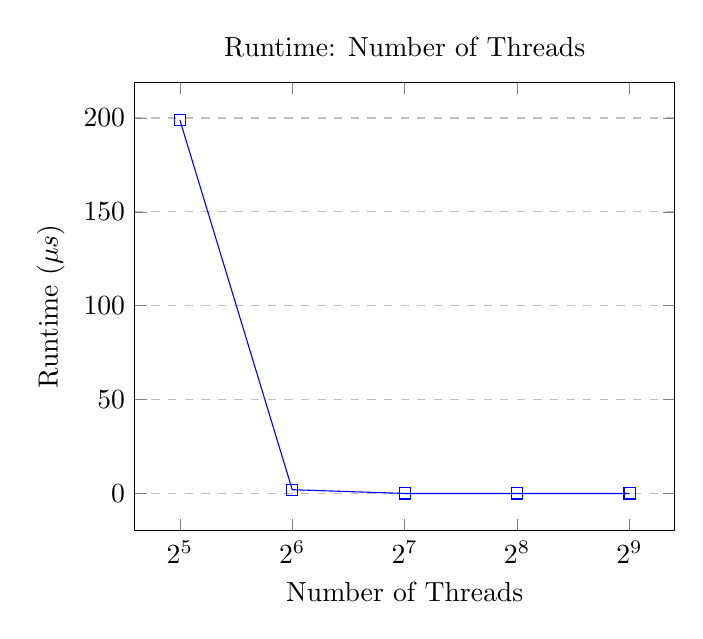
\begin{tikzpicture}
    \begin{axis}[
        title={Runtime: Number of Threads},
        xlabel={Number of Threads},
        ylabel={Runtime ($\mu s$)},
        %xmin=0, xmax=100,
        % ymin=0, ymax=200,
        xmode=log,
        log basis x=2,
        xtick={16,32,64,128,256,512},
        %ytick={0,20,40,60,80,100,120},
        legend pos=south east,
        ymajorgrids=true,
        grid style=dashed,
    ]
    
    \addplot[
        color=blue,
        mark=square,
        ]
        coordinates {
        (32,199)(64,2)(128,0)(256,0)(512,0)
        };
        
    \end{axis}
    \end{tikzpicture}
    \caption{Decrease of runtime with increasing number of used threads. It can be seen that increasing the number of threads drastically reduces computation time which is expected. It can also be seen, that for the given problem size, increasing the number of threads after a certain point does not lead to more efficiency. }
    \label{fig:threads}
\end{figure}


\section{Analysis}
If given the number of threads $T$ and single-core runtime $\tau$, it is expected to receive a time saving of $\frac{\tau}{T}$ for parallelizable as the work gets divided into $T$ equally sized work packages as \cite{opencsf} supports. Fig. \ref{fig:singlevmulti} shows that this holds roughly true, but can see that the real time saving is lower due to the overhead work. From the measurements we can infer that the overhead penalty scales significantly better than the single-core problem, as the efficiency gets better with increasing problem size, thus the overhead penalty becomes more and more diminishable. 

\section{Conclusion}
To conclude, parallelizing matrix-matrix multiplication has a significant advantage for runtime, scaling with the amount of available threads, limited by the problem size and the memory bandwidth. Achieving the same result is not possible with other paradigms. The closest paradigm would be threading. But as threading is more used for asynchronous tasks, which in application is usually not the case, the use of threading might only be useful in very specific, low power cases. 

This evidence so far has only described the linear part of an FFN-layer. To make an FFN-layer, a non-linear activation function is needed. This activation function is usually configured from the user and therefore not predetermined and can in theory be any kind of non-linear, single dimensional function (some other restrictions do apply, but are not important here) as described for example in \cite{Goodfellow-et-al-2016}. Thus, to make a fully functioning layer, the paradigm of functional programming is needed, to be enable the user to pass custom activation functions into the layer that can be the applied element-wise. This paradigm therefore can be used to extend this evidence.  

\bibliographystyle{apalike}
\bibliography{lib}
\end{document}


